% !TEX encoding = UTF-8
% !TEX TS-program = pdflatex
% !TEX root = ../tesi.tex

%**************************************************************
\chapter{Valutazione retrospettiva}
\label{cap:valutazione-retrospettiva}
%**************************************************************

\section{Raggiungimento degli obiettivi}
\subsection{Obiettivi aziendali}
%Breve bilancio sugli obiettivi raggiunti in rapporto a quelli preventivati.
Al termine del progetto di stage ho analizzato gli obiettivi raggiunti rispetto a quelli fissati inizialmente. Di seguito riporto una tabella con le valutazioni.

\renewcommand{\arraystretch}{1.4}
\begin{longtable}{|p{8cm}|p{2.5cm}|p{3cm}|}
\hline
\textbf{Obiettivo} & \textbf{Tipo} & \textbf{Esito finale} \\ 
\hline
Integrazione di un sistema completo per l'apertura di serrature con lettura di codice a barre e NFC & Obbligatorio & Soddisfatto \\ 
\hline
Realizzazione della piattaforma web per la gestione degli accessi & Obbligatorio & Soddisfatto \\ 
\hline
Creazione del modello 3D dell'involucro e sua realizzazione con stampa 3D & Obbligatorio & Soddisfatto \\ 
\hline
Redazione della manualistica completa & Obbligatorio & Soddisfatto \\ 
\hline
Cura e definizione dell'interfaccia grafica della piattaforma web & Desiderabile & Soddisfatto \\ 
\hline
Ottimizzazione del sistema esistente in termini di efficienza e prestazioni & Desiderabile & Non soddisfatto \\ 
\hline
Creazione di un modello 3D modulare espandibile per future versioni & Facoltativo & Non soddisfatto \\ 
\hline
\caption{Valutazione finale sugli obiettivi aziendali.}
\end{longtable}

Sono alcune le motivazioni per cui alcuni degli obiettivi prefissati non sono stati raggiunti:

\begin{itemize}
\item \textbf{Conoscenza limitata o assente}: per lo svolgimento del progetto di stage ho lavorato con nuove tecnologie e strumenti mai utilizzati prima d'ora. L'attività di studio iniziale è stata molto utile per l'apprendimento sul funzionamento di Arduino e la sua programmazione. Al contrario, il periodo di formazione personale precedente allo sviluppo non è stato sufficiente per un apprendimento esaustivo sul \textit{framework} Laravel. Questo ha comportato delle piccole attività di ricerca anche durante la codifica, rallentandola.

Analogamente, la conoscenza basilare del software Rhinoceros mi ha permesso di sviluppare solamente un modello base non espandibile per eventuali versioni future.
\item \textbf{Alternanza lavorativa}: essendo studente lavoratore, ho dovuto trovare un compromesso con il tutor aziendale per lo svolgimento dello stage: ho svolto le prime cinque settimane a tempo pieno fino al raggiungimento di 200 ore, mentre le rimanenti ore sono state suddivise su una base di 24 ore settimanali. Questa suddivisione ha compromesso l'attività di codifica, in quanto non ho potuto dare continuità al lavoro di sviluppo, rallentando, seppur in percentuale minima, la realizzazione del progetto.
\item \textbf{Mancanza di tempo}: a causa delle motivazioni sopra descritte, l'attività di codifica ha richiesto un tempo maggiore a quanto pianificato e pertanto il tempo a disposizione non è stato sufficiente per il raggiungimento di alcuni obiettivi.
\end{itemize}

\subsection{Obiettivi personali}
La valutazione sul rapporto tra gli obiettivi personali prefissati e quelli raggiunti porta al seguente risultato:

\begin{longtable}{|p{10.5cm}|p{3cm}|}
\hline
\textbf{Obiettivo} & \textbf{Esito finale} \\ 
\hline
Codifica e correlazione tra hardware e software & Soddisfatto \\ 
\hline
Modellazione e stampa 3D & Soddisfatto \\ 
\hline
Lavoro in team & Soddisfatto \\ 
\hline
Formazione lavorativa in ambito software & Soddisfatto \\ 
\hline
Accrescere le mie conoscenze & Soddisfatto \\ 
\hline
\caption{Valutazione finale sugli obiettivi personali.}
\end{longtable}

Sono riuscito a soddisfare tutti gli obiettivi prefissati prima dell'inizio dello stage, anche se alcuni con percentuale maggiore rispetto ad altri. Ad esempio, seppur avendo imparato le basi della modellazione e stampa 3D, avrei voluto poter approfondire ulteriormente lo studio, soprattutto per quanto riguarda la creazione di modelli tridimensionali.

La mia valutazione è comunque positiva, in quanto ho ottenuto una crescita di conoscenze e capacità in tutti gli aspetti.



\section{Bilancio formativo}

Al termine dello stage devo ritenermi soddisfatto rispetto alle aspettative iniziali di crescita personale. Questo progetto mi ha permesso di mettere in pratica buona parte delle conoscenze acquisite durante il mio percorso di studi e di arricchire la mia formazione con nuove tecnologie.

\begin{itemize}
\item \textbf{Interazione tra hardware e software}: prima dell'inizio dello stage era mio interesse imparare la programmazione hardware e comprendere come il software interagisce con le componenti elettroniche. A tirocinio terminato sono soddisfatto rispetto a quelle che erano le mie aspettative su questo punto: ho appreso il funzionamento di Arduino, strumento open source ormai largamente diffuso e utilizzato per la prototipazione rapida, la sua programmazione tramite l'IDE dedicato e alcune basi di elettronica.
\item \textbf{Modellazione e stampa 3D}: lo svolgimento di questo progetto mi ha permesso di conoscere il mondo della stampa 3D molto da vicino. A stage terminato ho acquisito delle utili competenze che variano dalla modellazione 3D alla stampa del modello.
\item \textbf{Sviluppo software in team}: durante il percorso universitario ho svolto progetti didattici, come ad esempio durante il corso di Ingegneria del Software, mirati a simulare nel modo più fedele possibile lo sviluppo di un software nel mondo del lavoro. Grazie allo stage, ho avuto la possibilità di confrontare quanto vissuto in ambiente universitario con le problematiche reali del mondo lavorativo. Questo implica interagire con un team di sviluppo eterogeneo, composto da sviluppatori con competenze e abilità a volte molto diverse.
\end{itemize}

Ho voluto tradurre in grafico l'andamento della mia conoscenza su alcuni aspetti e tecnologie, valutandone il cambiamento avvenuto al termine del progetto di stage.

\begin{figure}[H]
	\begin{center}
	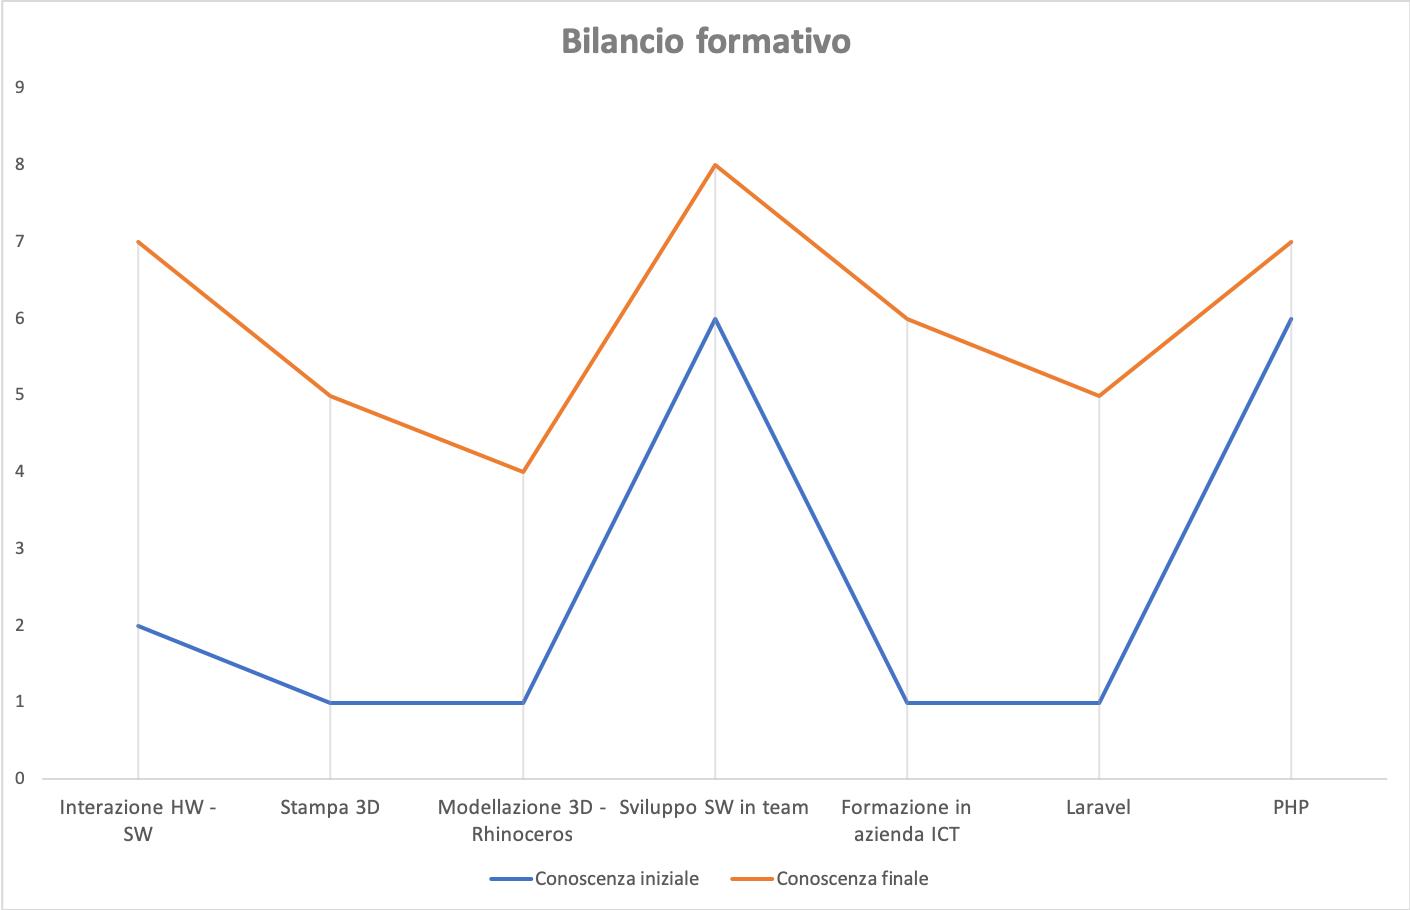
\includegraphics[scale=0.49]{immagini/bilancio_formativo.png}
	\caption{Grafico di confronto della conoscenza acquisita. La scala delle conoscenze va da 0 a 10. I dati sono stati ottenuti a seguito di un'autovalutazione.}
	\end{center}
\end{figure}

\section{Università e mondo del lavoro}
Il compito dell'Università non è limitato alla formazione di uno studente su vari fronti, ma si estende alla sua preparazione per affrontare l'inserimento al mondo del lavoro, al termine del percorso di studio. Questo non significa che uno studente laureato debba essere già in grado di svolgere un lavoro, ma deve essere preparato a superare le problematiche che gli si presentano. 

\medskip

Sulla base della mia esperienza, uno studente universitario, grazie alla preparazione ricevuta, è in grado di  gestire in autonomia il lavoro assegnatogli, sapendo affrontare anche situazioni impreviste. Inoltre possiede un'ottima capacità di adattamento rispetto allo studio di nuove tecnologie e all'utilizzo di nuovi strumenti di lavoro.

\medskip

Nella visione generale del corso di laurea in Informatica ritengo molto utile e stimolante per gli studenti l'utilizzo di progetti didattici, sia individuali che di gruppo, a supporto di alcuni corsi di studio. Ciò permette di mettere subito in pratica quanto si apprende durante le lezioni frontali, avendo al tempo stesso un obiettivo da portare a termine entro i tempi stabiliti e con le risorse a disposizione. A tal proposito, si potrebbero integrare alcuni corsi con un progetto didattico, come ad esempio il corso di Reti e Sicurezza, il quale tratta tematiche a mio avviso molto importanti per il mondo del lavoro.

Un possibile ampliamento potrebbe riguardare il corso di Basi di Dati inserendo la spiegazione di database \textit{NoSQL}, come ad esempio \textit{MongoDB}, attualmente in larga diffusione.
Manca inoltre un corso di studi che tratti lo sviluppo di applicazioni mobile iOS e Android, conoscenza molto richiesta nel mondo del lavoro.

\medskip

Un altro aspetto molto importante è lo stage che si svolge al termine del percorso di studio, dopo il completamento di tutti gli esami previsti dal corso di studi. Collocare lo stage anticipatamente andrebbe a discapito dello studente, il quale potrebbe non avere le conoscenze necessarie ad affrontare il progetto. Inoltre la propedeuticità data dall'insegnamento di Ingegneria del Software fornisce allo studente l'esperienza necessaria allo svolgimento di un progetto software in autonomia. Detto ciò, ritengo altrettanto utile l'inserimento di un progetto antecedente lo stage che potrebbe essere di tre tipologie:
\begin{itemize}
\item \textbf{Stage ridotto}: un tirocinio in forma ridotta rispetto a quello di fine studi, ma con la finalità di inserire lo studente nell'ottica lavorativa;
\item \textbf{Workshop estivi}: organizzare progetti di fine anno dove gli studenti raccolti in gruppi devono sviluppare progetti mettendo in pratica tutte le conoscenze apprese durante i corsi svolti nell'anno accademico;
\item \textbf{Hackathon}: creare un evento al termine dell'anno accademico mirato alla competizione tra gli studenti. Il tema proposto potrebbe trattare argomenti studiati durante i corsi.
\end{itemize}

Ritengo che tali iniziative potrebbero aumentare l'interesse degli studenti e stimolarli andando ad aumentare la produttività.